\phantom{.}
	
\ClearShipoutPicture 
\AddToShipoutPicture{%
 	\AtPageLowerLeft{\includegraphics[width=\paperwidth,height=\paperheight,page=8]{../notext_lb.pdf}}
}

\placetextbox{0.1}{0.935}{.5\paperwidth}{\centering
\textrm{\fontsize{30}{1} \ding{66}} \kern-.5cm
{\fontsize{33}{1} \textsc{ The Owl }} \kern-.5cm
\textrm{\fontsize{30}{1} \ding{66}}}
	\placetextbox{0.1}{0.9}{.5\paperwidth}{\fontsize{15}{1}\centering \textit{An old but reliable skyship, outfitted for smuggling}}

	
	\placetextbox{0.655}{0.67}{\paperwidth}{\fontsize{13}{0}\fontcelestiaantiqua\scshape relative size comparison}
	\placetextbox{0.58}{0.605}{\paperwidth}{
\fontsize{11}{0}\fontcelestiaantiqua\scshape the owl
{\fontsize{9}{0}\fontcelestiaantiqua \ding{226}}
48m}
	\placetextbox{0.745}{0.605}{\paperwidth}{
\fontsize{11}{0}\fontcelestiaantiqua\scshape sky squid
{\fontsize{9}{0}\fontcelestiaantiqua \ding{226}}
139m}
	\placetextbox{0.61}{0.52}{\paperwidth}{
\fontsize{11}{0}\fontcelestiaantiqua\scshape hand of sorrow
{\fontsize{9}{0}\fontcelestiaantiqua \ding{226}}
550m}
	
	\placetextbox{0.089}{0.455}{0.4\paperwidth}{\fontsize{9}{12}\fontcelestiaantiqua
{\textsc{\fontsize{14}{0}\fontcelestiaantiqua \phantom{.....} Sky Hauler C9 Refit}} \vspace{4pt} \\
\phantom{..} \textit{The Owl} was once a Sky Hauler C9 cargo ship but has since
been extensively customized by Cyrus and Kale. It has a smaller
cargo area and four passenger berths in the reclaimed space. It
also has hidden smuggling compartments scattered throughout
the vessel. \vspace{5pt} \\
\textit{The Owl} is an old ship, but it can hold its own with more modern
vessels thanks to its custom engines and supercharged steam
drive. Snargle has also made several unique adjustments to the
controls to allow the large ship to maneuver like a much smaller
craft. \vspace{5pt} \\
Unfortunately, all of these modifications put a lot of strain on the
old girl. Kale keeps the ship running day to day, but when it’s put
under a lot of stress (as it often is) things can go awry—broken
pipes, vented steam, leaking fluids, and worse. \vspace{5pt} \\
Still, \textit{The Owl} is not just a skyship, it’s a home to its crew. They
gather around the beat-up old wooden dinner table in the galley
every night and thank the four winds that fortune saw fit to bless
them with such a fine craft. \vspace{10pt} \\
{[GM: You can inflict conditions on \textit{The Owl} as events warrant. It begins
play with the \textbf{Need Fuel} condition marked.]}
}
	\placetextbox{0.51}{0.46}{0.4\paperwidth}{\fontsize{10}{12}\fontcelestiaantiqua
{\fontsize{14}{0} \textsc{Statistics}} \vspace{4pt} \\
Length: 48 meters \vspace{5pt} \\
Crew: 2–3 \vspace{5pt} \\
Berths: 6 (2 crew, 4 passenger) \vspace{5pt} \\
Cargo Capacity: 30,000 pounds (6 cargo pods) \vspace{5pt} \\
Powerplant:
\begin{itemize}[noitemsep,topsep=3pt]
	\item Tri-Valve Reciprocal Steam Drive 
	\item (2) Twin-Coil Induction Thrusters
\end{itemize} \vspace{5pt}
Cruise Speed: 160 knots \vspace{5pt} \\
Flank Speed: 310 knots under boost \vspace{5pt} \\
Weapons: Top-mounted external gun turret \vspace{5pt} \\
Wireless: Midrange Multi-Band with Signal Mask \vspace{5pt} \\
Sensors:
\begin{itemize}[noitemsep,topsep=3pt]
	\item Short-Range Sonar 
	\item Atmosphere/Pressure Analyzer
\end{itemize} \vspace{5pt}
Hull: Treated to resist corrosion in the lower depths for up to 4
hours.
}


\placetextbox{0.156}{0.0875}{0.2\paperwidth}{\fontsize{12}{0}\fontcelestiaantiqua\scshape need fuel}
\placetextbox{0.298}{0.0875}{0.2\paperwidth}{\fontsize{12}{0}\fontcelestiaantiqua\scshape need supplies}
\placetextbox{0.4735}{0.0875}{0.2\paperwidth}{\fontsize{12}{0}\fontcelestiaantiqua\scshape busted \kern-2pt \& \kern-2pt leaking}
\placetextbox{0.6835}{0.0875}{0.2\paperwidth}{\fontsize{12}{0}\fontcelestiaantiqua\scshape slowed}
\placetextbox{0.798}{0.0875}{0.2\paperwidth}{\fontsize{12}{0}\fontcelestiaantiqua\scshape crippled}